\documentclass[12pt,a4paper]{article}
\usepackage{url}
\usepackage[backend=bibtex]{biblatex}
\usepackage{caption}
\usepackage[utf8]{inputenc}
\usepackage{enumerate}
\usepackage{tabularx}
\usepackage{graphicx}
\usepackage{float}
\usepackage{color}
\usepackage{amssymb,amsmath,wasysym}

\addbibresource{bib1.bib}

\begin{document}

\title{Computational Intelligence, SS2017, Assigment 3}

\author{%
\name{Lucas Reeh}
\email{lreeh@student.tugraz.at}
}
\date{\today}

\begin{titlepage}
   \begin{center}
     \begin{huge}
		   %% Update assignment number here
           \textbf{Assignment 3}
     \end{huge}
   \end{center}

   \begin{center}
     \begin{large}
           Computational Intelligence, SS2017
     \end{large}
   \end{center}

   \begin{center}
 \begin{tabularx}{\textwidth}{|>{\hsize=.33\hsize}X|>{\hsize=.33\hsize}X|>{\hsize=.33\hsize}X|} 

           \hline
           \multicolumn{3}{|c|}{\textbf{Team Members}} \\
           \hline
           Last name & First name & Matriculation Number \\
           \hline
           Reeh & Lucas & 00630128 \\
           \hline

     \end{tabularx}
   \end{center}
\end{titlepage}

\tableofcontents
\listoffigures

\newpage

\section{1}

\subsection{1.1}

\begin{enumerate}[a)]
  
%%%%%%%%%%%%%%%%%%%%%%%%%% 1.1 a)
  
  \item \textbf{1.1 a}
  
Following plots show the learned function after ``fitting'' data sets to neural
network Python scikit-learn\autocite{scikit} using different numbers of neurons
in 1 hidden layer in den netowrk.
  
\begin{figure}[H]
	\centering
  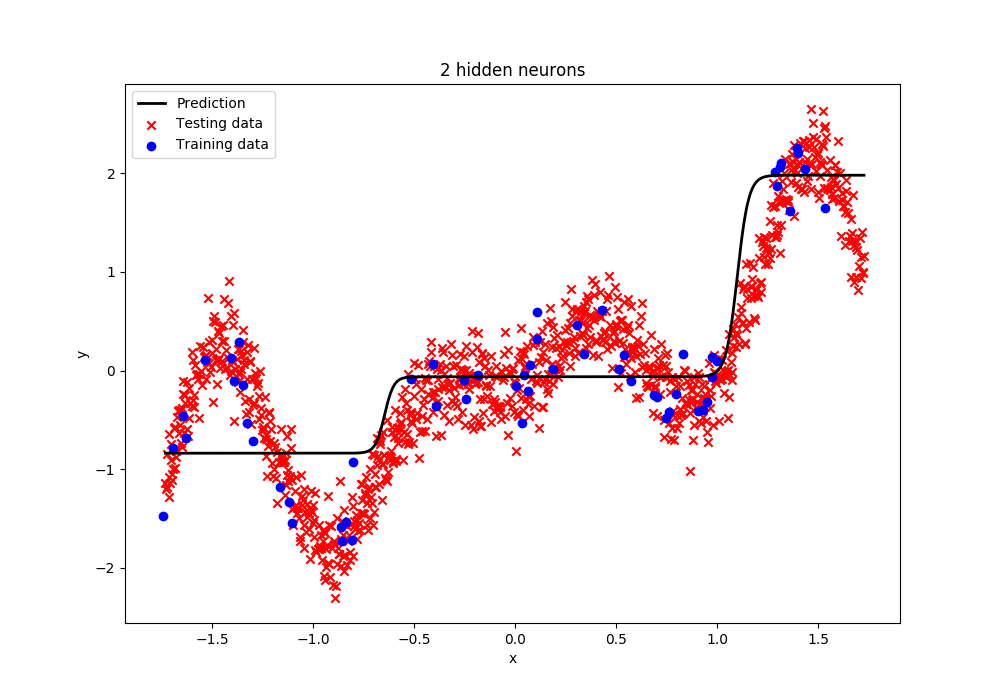
\includegraphics[width=0.9\textwidth]{figures/1_1_a_hn_2.png}
	\caption{NN Learned function $h_n=2$}
	\label{1_1_a_hn_2}
\end{figure}

\textbf{Discussion}

$2$ ``neurons'' in the hidden layer are cleary an underfitting parametrization
(missing a lot of data points), $h_n = 8$ seems to miss data points where $ x =
0.0$, $40$ nodes tend to overfit a little (see slope around $x = 1.5$ is going
up again). As shown in Figure \ref{1_1_a_hn_100} $100$ hidden layers seem to
recognize the concarve slope around $x = 0.0$ but is also overfitting at $x >
1.2$. From this Traning data there is no saying if this curve should be added. I
added it just because it is possible.

\begin{figure}[H]
	\centering
  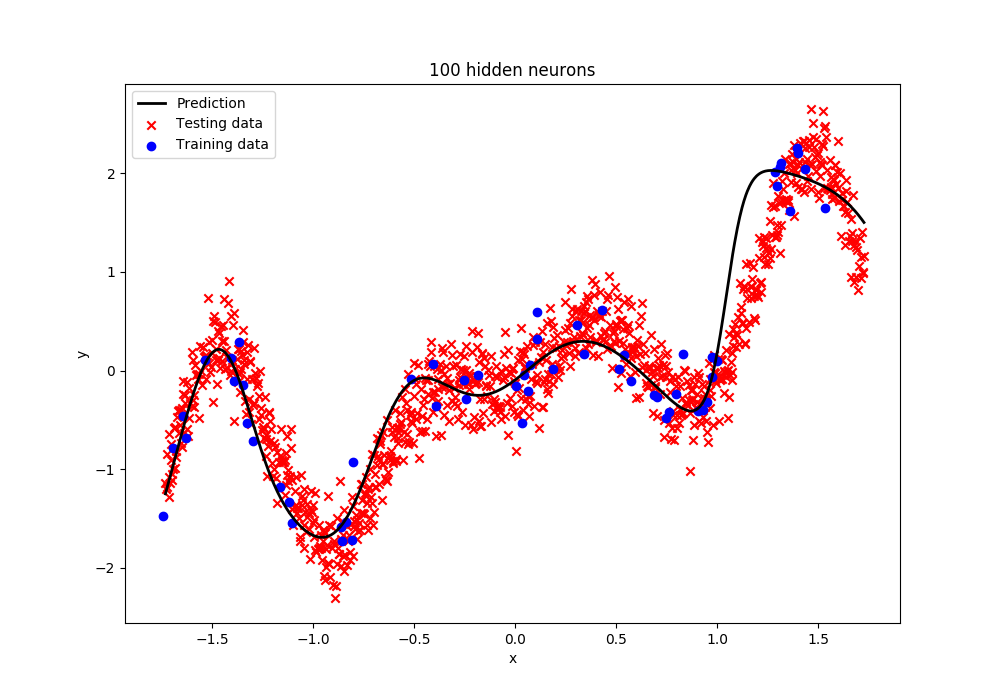
\includegraphics[width=\textwidth]{figures/1_1_a_hn_100.png}
	\caption{NN Learned function $h_n=100$}
	\label{1_1_a_hn_100}
\end{figure}

\end{enumerate}

\newpage
\printbibliography

\end{document}